\documentclass[11pt]{scrartcl}
\usepackage[utf8]{inputenc}
\usepackage[sexy]{evanchen} 
\usepackage{graphicx}
\graphicspath{{8 Outsource K Math/Gambar/}}

\title{Symmedian}
\author{Azzam and Akeyla}

\begin{document}

\maketitle

\renewcommand*\contentsname{Daftar Isi}
\tableofcontents

\newpage

\section{Definisi}
$A-$symmedian dari sebuah segitiga $ABC$ merupakan pencerminan garis berat (median) dari titik $A$ terhadap garis bagi dalam dari titik $A$.
\begin{figure}[h]
    \centering
    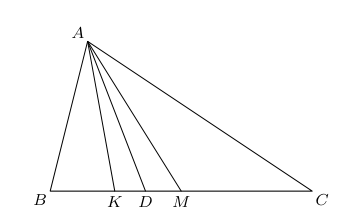
\includegraphics[width=0.5\linewidth]{SymmedianDef.png}
    \caption{$AM, AD, AK$ secara berturut-turut adalah garis berat, garis bagi dalam, dan symmedian dari titik $A$}
    \label{fig:symm-def}
\end{figure}

\section{Properti}
\begin{lemma}
    Symmedian dari titik $A$, $B$, dan $C$ berpotongan di satu titik.
\end{lemma}

\begin{proof}
    Gunakan ceva trigonometri
\end{proof}

Titik perpotongan ketiga symmedian dari segitiga $ABC$ disebut sebagai titik symmedian atau titik Lemoine.

\begin{lemma}
    Misal garis singgung dari lingkaran luar $ABC$ di titik $A$ dan $B$ berpotongan di $P$. Maka, $AP$ adalah $A-$symmedian dari segitiga $ABC$.
\end{lemma}

\begin{proof}
    Tinjau lingkaran $\omega$ yang berpusat di $P$ dan melewati $B$ dan $C$. Misal $D = AB \cap \omega$ dan $E = AC \cap \omega$. Amati bahwa $ADE$ sebangun dengan $ACB$. Lebih lanjut, dapat dibuktikan dengan angle chasing bahwa $\angle{DBE} = 90^{\circ}$ sehingga $DE$ adalah diameter dan $P$ adalah titik tengah $DE$. Jadi, $AP$ adalah symmedian.
\end{proof}

\begin{lemma}
    Jixa $K$ adalah perpotongan $A-$symmedian dengan $BC$, maka didapat \[\dfrac{BK}{CK} = \dfrac{AB^2}{AC^2}\]
\end{lemma}

\begin{proof}
    Gunakan dalil sinus pada segitiga $ABK$ dan $ACK$
\end{proof}

\begin{definition}
    Dua garis $l_1$ dan $l_2$ disebut antiparallel terhadap sudut $\theta$ apabila pasangan sudut yang terbentuk antara perpotongan sudut tersebut dengan kedua garis sama tetapi posisinya terbalik.
\end{definition}

\begin{figure}[h]
    \centering
    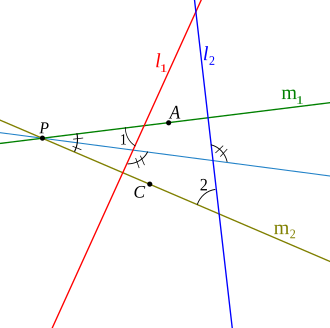
\includegraphics[width=0.5\linewidth]{antiparallel.png}
    \caption{Garis $l_1$ dan $l_2$ antiparallel terhadap sudut $\angle{APC}$}
    \label{fig:anti-parallel}
\end{figure}

\begin{lemma}
    $A-$symmedian adalah lokus dari semua titik tengah garis yang antiparallel terhadap $\angle{BAC}$
\end{lemma}

\begin{proof}
    Gunakan Generalized Angle Bisector Theorem
\end{proof}

\section{Latihan}
\begin{problem}
    (Turki MO 2004) Di sebuah segitiga $ABC$ dengan $\angle B > \angle C$, garis tinggi, garis bagi dalam, dan garis berat dari titik $A$ memotong $BC$ secara berturut-turut di titik $H, L,$ dan $D$. Buktikan bahwa $\angle{HAL} = \angle{DAL}$ jika dan hanya jika $\angle{BAC} = 90^{\circ}$. \textbf{Hint: Inggris}
\end{problem}

\begin{problem}
    (Siprus IMO TST 2 2022) $ABC$ merupakan segitiga tumpul dengan $\angle{ABC} > 90^{\circ}$ dan $c$ adalah lingkaran luarnya. Garis bagi dalam sudut $\angle{BAC}$ memotong $c$ lagi di titik $E$ dan memotongan $BC$ di titik $D$. Lingkaran berdiameter $DE$ memotong $c$ di titik $H$. Jika garis $HE$ memotong garis $BC$ di titik $K$, buktikan bahwa:
    \begin{enumerate}
        \item Titik $K, H, D,$ dan $A$ konsiklik
        \item Garis $AH$ melewati titik perpotongan garis singgung $c$ pada titik $B$ dan $C$
    \end{enumerate}
    \textbf{Hint: Argentina, Inggris}
\end{problem}

\begin{problem}
    (Lingkaran Lemoine Pertama) $K$ adalah titik symmedian dari segitiga $ABC$. Buktikan bahwa keenam titik perpotongan ketiga garis yang sejajar dengan masing-masing sisi $ABC$ dengan dua sisi lainnya akan konsiklik. \textbf{Hint: Somalia}
\end{problem}

\begin{problem}
    (Lingkaran Lemoine Kedua) $K$ adalah titik symmedian dari segitiga $ABC$. Buktikan bahwa keenam titik perpotongan ketiga garis yang antiparallel dengan masing-masing sisi $ABC$ dengan dua sisi lainnya akan konsiklik. \textbf{Hint: Islandia}
\end{problem}

\begin{problem}
    (Polandia MO 2000) Diberikan sebuah segitiga $ABC$ yang memenuhi $AC = BC$. Titik $P$ terletak di interior segitiga $ABC$ sedemikian hingga $\angle{PAB} = \angle{PBC}$. Notasikan $M$ sebagai titik tengah $AB$. Buktikan bahwa $\angle{APM} + \angle{BPC} = 180^{\circ}$. \textbf{Hint: Polandia}
\end{problem}

\begin{problem}
    (Pan-African MO 2013) $ABCD$ adalah sebuah segiempat konveks dengan $AB$ sejajar $CD$. Titik $P$ dan $Q$ secara berturut-turut merupakan titik tengah $AC$ dan $BD$. Buktikan bahwa jika $\angle{APB} = \angle{CBD}$ maka $\angle{BCQ} = \angle{ACD}$.
    \textbf{Hint: Mesir}
\end{problem}

\begin{problem}
    (Meksiko MO 2000) Diberikan segitiga tumpul $ABC$ dengan $\angle B > 90^{\circ}$. Titik $H$ ada di sisi $AC$ sedemikian hingga $AH = BH$ dan $BH$ tegak lurus dengan $BC$. Titik $D$ dan $E$ secara berturut-turut adalah titik tengah $AB$ dan $BC$. Garis yang melewati $H$ dan sejajar dengan $AB$ memotong $DE$ pada titik $F$. Buktikan bahwa $\angle{BCF} = \angle{ACD}$
    \textbf{Hint: Honduras, Kuba}
\end{problem}

\newpage
\section{Hint}
\begin{enumerate}
    \item (Buenos Aires) Angle chasing
    \item (Cairo) Tinjau perpotongan $AC$ dan $BD$
    \item (Havana) Tinjau $C-$symmedian
    \item (London) $AH$ adalah symmedian
    \item (Mogadishu) Misal $P_3$ dan $Q_3$ secara berturut-turut adalah perpotongan garis yang sejajar terhadap $AB$ dengan $AC$ dan yang sejajar terhadap $AC$ dengan $AB$. Segiempat apakah $AP_3KQ$ itu?
    \item (Reykjavik) Tinjau titik tengah keenam segmen garis yang antiparallel tersebut.
    \item (Tegucigalpa) Segiempat apakah $HDBF$ itu?
    \item (Warsaw) Tinjau lingkaran luar $APB$
\end{enumerate}

\end{document}